% !TeX root = ../msc_thesis_jayd.tex
\chapter{Numerical Tools}

\section{Numerical Computation of the Scattering Matrix}\label{sec:app.numTools.scatMat}
We detail the numerical solution of Helmholtz's equation with the onion discretization 
procedure of \gls{sqa}.

In the TE case, we must take $n\mapsto n_\text{eff}$. This leads us to evaluate the 
extra integral
  \begin{equation}
   I = \frac{1}{2\pi}\int_0^{2\pi}\left[\frac{1}{n}\frac{d^2n(r_j,\theta)}{d\theta^2}-\frac{2}{n^2}\left(\frac{dn(r_j,\theta)}{d\theta}\right)^2\right]e^{i(m-m')\theta}d\theta.
  \end{equation}
The numerical cost of this integral can be lessened 
if we notice that if we write it as a function of $n^2$ we obtain
  \begin{equation}
   I = \frac{1}{2\pi}\int_0^{2\pi}\left[\frac{1}{2n^2}\frac{d^2n^2(r_j,\theta)}{d\theta^2}-\frac{3}{4n^4}\left(\frac{dn^2(r_j,\theta)}{d\theta}\right)^2\right]e^{i(m-m')\theta}d\theta
  \end{equation}
which, in turn, can be rewritten as
  \begin{equation}
   I = \frac{1}{2\pi}\int_0^{2\pi}\left[\frac{1}{2}\frac{d^2\log n^2(r_j,\theta)}{d\theta^2}-\left(\frac{1}{2}\frac{d\log n^2(r_j,\theta)}{d\theta}\right)^2\right]e^{i(m-m')\theta}d\theta.
  \end{equation}
Integrating by parts twice yields
  \begin{equation}
   I = \frac{1}{2\pi}\int_0^{2\pi}\left[-\frac{(m-m')^2}{2}\log n^2(r_j,\theta)-\left(\frac{1}{2}\frac{d\log n^2(r_j,\theta)}{d\theta}\right)^2\right]e^{i(m-m')\theta}d\theta.
  \end{equation}
The second term cannot be integrated out, but this final result means that
we will only need to numerically evaluate the first derivative of the 
refractive index (although its analytical form could be provided).

Notice the form of the $\mat{L}^j$ matrix. As can be seem from inspection, 
the value of the elements depend only on their distance from the diagonal.
Taking a closer look reveals the form
  \begin{equation}
   \mat{L}^j = \mat{M}^2 +k^2r_j^2\begin{pmatrix} 
		  n_0 & n_{-1} & \cdots & \cdots & n_{-2M}	\\
		  n_1	  & n_0& \cdots & \cdots & n_{-2M-1}\\
		  n_2	  & n_1	   & n_0& \cdots & n_{-2M-2}\\
		  \vdots  & n_2    & n_1    & \ddots & \vdots   \\
		  n_{2M}  & \cdots & \cdots & \cdots & n_0
		\end{pmatrix}
  \end{equation}
which is manifestly Toeplitz. When the potential is real, the Fourier
series has the property $n_{-j}=n_j^*$, which makes the $\mat{L}^j$ 
matrix Hermitian. In the general case, however, it is not. Because
we will need to use orthogonality relations in what follows, we must
compute both the left and right eigenvectors\index{left eigenvectors}. 
We will note the left (covariant) basis by $\Ket{\tilde{\Phi}_\mu^j}$.
This is not sufficient, however, because we are not guaranteed that
both sets of eigenvectors will form a complete basis. 

\paragraph{Normality of $\mat{L}^j$}


\section{Computation of the Logarithmic Derivative $[H^{(\pm)}_\nu(z)]'/H^{(\pm)}_\nu(z)$}\label{sec:app.numTools.logDeriv}

\index{continued fraction expansions|(textbf}
As we have seen from Appendix \ref{app:basicEquations}, the computation of the logarithmic derivative
of Bessel functions is of the utmost importance in the numerical solution 
of scattering problems. Given that we already use Amos' library \cite{AMO86} to evaluate
the Bessel functions, we might have been tempted to use it 
to directly evaluate the derivative. It turns out that using
expansions that pertain to logarithmic derivatives is somewhat
faster and is more accurate than using Amos' library. 

In this section, we introduce some concepts relating to 
continued fraction expansions (CFEs) and discuss their numerical
evaluation. We then derive the CFEs and other expansions that will
be of use in the computation of the logarithmic derivatives.

\subsection{Notation and Necessary Theorems}
A continued fraction expansion is a representation
of a mathemetical function. It can be linked to 
Laurent series, Padé approximants and much more 
\cite{CUY2008}. It has the standard form 
  \begin{equation}
    f = b_0+\cfrac{a_1}{b_1+\cfrac{a_2}{b_2+\cfrac{a_3}{b_3+\cfrac{a_4}{b_4+\cdots}}}}
  \end{equation}
or, more succinctly, 
  \begin{equation}
   f = b_0 + \bigk_{m=1}^\infty\left(\frac{a_m}{b_m}\right)
  \end{equation}
where 'K' is for the German word \textit{Kettenbruch}, meaning continued fraction.
We define the $n$th approximant as
  \begin{equation}
   f_n = b_0 + \bigk_{m=1}^n\left(\frac{a_m}{b_m}\right).
  \end{equation}
We will be concerned with their numerical evaluation and convergence properties.

\index{continued fraction expansions!numerical evaluation of}
Notice that naïvely evaluating the CFE from right-to-left, as a person would do, 
does not yield a satisfying numerical algorithm, as the amount of iterations 
must be fixed in advance and consequently does not allow the control the 
accuracy of the evaluation. The chosen method is taken from the Holy Bible
of Numerics, \textit{Numerical Recipes} \cite{PRE2007} and is called 
the modified Lentz's method. It constructs a rational approximation
of the $n$th approximant 
  \begin{equation}
    f_n = \frac{A_n}{B_n}
  \end{equation}
where 
  \begin{align}
   A_{-1} 	&=1 			& B_{-1} 	&=0	\nonumber\\
   A_0		&= b_0			& B_0		&=1	\\
   A_j		&=b_jA_{j-1}+a_jA_{j-2}	& B_j 		&=b_jB_{j-1}+a_jB_{j-2}.\nonumber
  \end{align}
This method can lead to over/underflow of the floating-point representation: 
the method hence uses 
  \begin{align}
    C_j &= A_j/A_{j-1}			&	D_j	&= B_{j-1}/B_j	\nonumber\\
    	&= b_j+\frac{a_j}{C_{j-1}}	&		&= \frac{1}{b_j+a_jD_{j-1}}\\
    f_j	&= f_{j-1}C_jD_j.\nonumber
  \end{align}
The method is aptly described by Algorithm \ref{algo:app.numTools.cfeEvaluation}.
It allows for a left-to-right evaluation of the CFE and control of the relative
accuracy of the computation. 

  \begin{algorithm}
   \KwData{\texttt{tiny} = square root of smallest representable number}
   \KwData{\texttt{eps} = accuracy of the CFE}
   \eIf{$b_0 = 0$}{$f_0\leftarrow$\texttt{tiny}}{$f_0\leftarrow0$}
   $C_0 \leftarrow f_0$\;
   $D_0 \leftarrow 0$\;
   \Repeat( from $j=1$){$|\Delta_j-1|<$\texttt{eps}}%
   {
    $D_j \leftarrow b_j+a_jD_{j-1}$\;
    \If{$D_j=0$}{$D_j\leftarrow$\texttt{tiny}}
    $C_j \leftarrow b_j+\frac{a_j}{C_{j-1}}$\;
    \If{$C_j=0$}{$C_j\leftarrow$\texttt{tiny}}
    $D_j \leftarrow 1/D_j$\;
    $\Delta_j\leftarrow C_jD_j$\;
    $f_j \leftarrow f_{j-1}\Delta_j$
   }
   \Return{$f_j$}
  \caption{Evaluation of Continued Fractions}
  \label{algo:app.numTools.cfeEvaluation}
  \end{algorithm}

As for the convergence properties, we will only bother with CFEs 
originating from three-term recurrence relations. Indeed, it turns out
that any three-term recurrence relation can be linked to a CFE. 
Consider  
  \begin{equation}
    \label{eq:app.numTools.threeTermRecurrence}
   y_{n+1} + a_ny_n + b_ny_{n-1} = 0. 
  \end{equation}
It can be rewritten as
  \begin{equation}
    \frac{y_n}{y_{n-1}} = -\frac{b_n}{a_n+y_{n+1}/y_n}.
  \end{equation}
Iterating yields the CFE
  \begin{equation}
   \label{eq:app.numTools.recurrenceCFE}
   \frac{y_n}{y_{n-1}} = \bigk_{m=n}^\infty\left(\frac{-b_m}{a_m}\right).
  \end{equation}
Given our goal of computing $[H^{(\pm)}_\nu(z)]'/H^{(\pm)}_\nu(z)$
and in light of (ref to recurrence relation of Bessel functions), it seems that
we have won. The next theorem, however, will prove us wrong.
   \begin{thm}[Pincherle's Theorem \cite{CUY2008}]
    If there exists a \textit{minimal solution} $u_n$ of the three-term
    recurrence relation \eqref{eq:app.numTools.threeTermRecurrence}, 
    the associated CFE \eqref{eq:app.numTools.recurrenceCFE} converges
    to $u_n/u_{n-1}$. A solution is said minimal if there exists another
    solution $v_n$ such that
      \begin{equation}
       \lim_{n\rightarrow\infty} \frac{u_n}{v_n} = 0.
      \end{equation}
    $v_n$ is said to be the dominant solution. The minimal solution is unique. 
   \end{thm}

Because the minimal solution of \eqref{eq:app.Bessel.recurrenceBessel} if $J_\nu(z)$, 
we cannot use the associated CFE to compute the logarithmic derivatives
of Hankel functions. Instead, we must look into the links between
Hankel functions and confluent hypergeometric functions. 

\subsection{CFE and Other Expansions}
In this brief foray into the vast subject
of hypergeometric functions, we will introduce Kummer's 
function and its link to the evaluation of the logarithmic
derivative.

Kummer's function solves the differential equation \cite[\S13.1.1]{ABR1965}
  \begin{equation}
    z\frac{d^2y}{dz^2}+(b-z)\frac{dy}{dz}-ay=0
  \end{equation}
and is noted $U(a,b,z)$. It can be shown that that $u_k=(a)_kU(a+k,b,z)$
is the minimal solution of the recurrence \cite{TEM1983}
  \begin{equation}
    u_{n+1} = \frac{2a-b+2n+z}{a-b+n+1}u_n - \frac{a+n-1}{a-b+n+1}u_{n-1}
  \end{equation}
where $(a)_k$ is the Pochhammer symbol. We can hence derive
  \begin{equation}
    \frac{U(a,b,z)}{U(a+1,b,z)} = 2a-b+2+z-\bigk_{m=1}^\infty\left(\frac{(a+m)(b-a-m-1)}{b-2a-2m-2-z}\right).
  \end{equation}
Combined with \cite[\S13.4.23]{ABR1965}
  \begin{equation}
    U(a+1,b,z) = \frac{1}{1+a-b}U(a,b,z) + \frac{z}{a(1+a-b)}U'(a,b,z), 
  \end{equation}
we obtain \cite{CUY2008}
  \begin{equation}
    \frac{dU(a,b,z)/dz}{U(a,b,z)} = -\frac{a}{z}+\frac{a(1+a-b)/z}{2a-b+2+z}_{-}\bigk_{m=1}^\infty\left(\frac{(a+m)(b-a-m-1)}{b-2a-2m-2-z}\right).
  \end{equation}
Given the relation between Kummer's functions and Hankel functions $H^\omega_{\nu}(z)$ \cite[\S13.6.22/23]{ABR1965}
  \begin{equation}
    H^\omega_\nu(z) = \frac{2}{\sqrt{\pi}}e^{-\omega\left[\pi\left(\nu+1/2\right)-z\right]}(2z)^\nu U(\nu+1/2,2\nu+1,-2i\omega z)\qquad (\omega=\pm)
  \end{equation}
we can finally find the CFE
  \begin{equation}
    \label{eq:app.numTools.cfeHankel}
    \frac{dH^\omega_\nu(z)/dz}{H^\omega_\nu(z)} = -\frac{1}{2z}+i\omega+\frac{\omega}{z}\bigk_{m=1}^\infty\left(\frac{\nu^2-(2m-1)^2/4}{2(iz-\omega m)}\right).
  \end{equation}
In our numerical implementation (see next section), we have found that when $|z|<10^{-2}$, convergence is slow. This mirrors the results of \cite{THO1986}.
We thus use the small argument expansions for the Bessel functions (\textit{q.v.} \S \ref{sec:app.Bessel.smallArguments}) to obtain
  \begin{subequations}
  \begin{align}
   \lim_{z\rightarrow0}\frac{dH^\omega_\nu(z)/dz}{H^\omega_\nu(z)}	&= -\frac{\nu}{z}	& (\nu\neq0)	\\
									&= \frac{1}{z}\left[\frac{\pi}{2i\omega}+\gamma+\ln\left(\frac{z}{2}\right)\right]^{-1} & (\nu=0).
  \end{align}
  \end{subequations}

\index{continued fraction expansions|)textbf}

\subsection{Numerical Tests}
We have performed a number of tests to ascertain the performance of our algorithm. 
To test the precision of the algorithm, we have evaluated the CFE for $z\in\{0,10\}$
and $\nu\in\{-100,100\}\in\mathbb{N}$ and compared it to the values obtained via
Amos' library for a range of tolerances. It can be seen that the maximum deviation 
decreases until our set tolerance hits $10^{-12}$ and then plateaus. Because 
convergence of \ref{eq:app.numTools.cfeHankel} is mathematically insured, we 
conclude that Amos's library evaluate the logarithmic derivative up to 
a precision of $10^{-12}$. This is probably due to the propagation 
of errors in the floating point operations, as we use relation
\eqref{eq:app.Bessel.recurrenceDiffBessel}
to evaluate the derivative. 

\begin{figure}
 \centering
 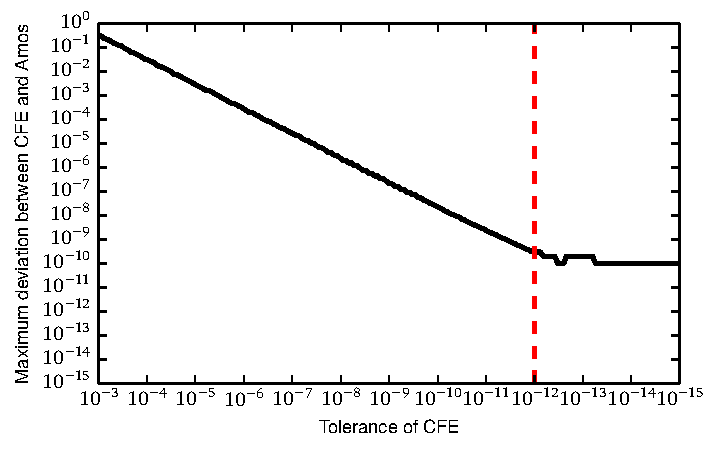
\includegraphics[width=0.7\textwidth]{figs/app-numTools/maxDiff.pdf}
 \caption[Maximum deviation between the CFE and Amos' implementation as a function
	  of the CFE tolerance]%
	 {Maximum deviation between the CFE and Amos' implementation of the Bessel functions
	 as a function of the tolerance of the CFE. This study was performed in the parameter
	 space $z\in\left\{0.1,10\right\}, \nu\in\left\{-100,100\right\}$. We interpret 
	 the plateau in maximum deviation as the error committed by Amos' implementation, i.e.
	 Amos' implementation has a precision of $\sim10^{-10}$ on the evaluation of the logarithmic derivative.}
\end{figure}


\begin{figure}
 \centering
 \begin{subfigure}[t]{0.47\textwidth}
  \centering
  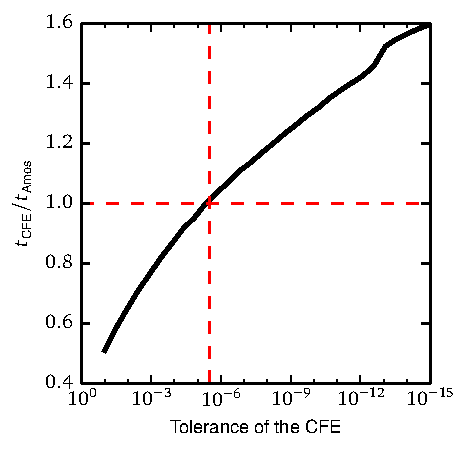
\includegraphics[width=\textwidth]{figs/app-numTools/timesTolerance.pdf}
  \caption{Performance of the CFE implementation as a function of its tolerance.
	   We measured the ratio of the time it takes to compute the logarithmic derivative
	   at $z=0$ for all orders $\nu\in\{-100,100\}$ with the CFE and Amos' implementation. 
	   When the tolerance of the CFE hits $\sim10^{-5.5}$, the CFE is slower than Amos'
	   implementation.}
 \end{subfigure}
 \begin{subfigure}[t]{0.47\textwidth}
  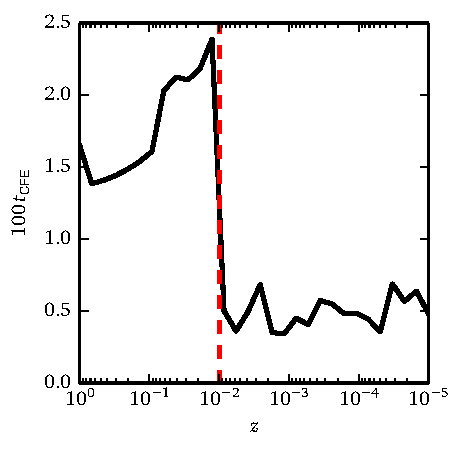
\includegraphics[width=\textwidth]{figs/app-numTools/timesPerformance.pdf}
  \caption{Performance of the CFE as a function of $z$. When approaching
  $z=0$ (from all sides), it takes a higher number of terms for the 
  CFE to converge, resulting in a slower algorithm. However, at $z=10^{-2}$, we 
  use the small argument form, preserving both precision and performance.}
 \end{subfigure}
 \caption[Performance of the CFE compared to Amos' library's.]
	 {Performance of the CFE compared to that of Amos' library. The CFE is somewhat
	 slower, but can achieve better precision.}
\end{figure}


However, it can be seen that Amos' library is somewhat faster, given its
precision, that our CFE evaluation 
even though it requires three Hankel function evaluations. 

%\section{Clebsch-Gordan Coefficients and Wigner Symbols}
\section{Wigner Symbols}\label{sec:app.wignerSymbols}
Before discussing the Wigner symbols, we introduce the Clebsch-Gordan
coefficients as they appear quite naturally in the quantum theory
of angular momentum. Specifically, they are needed to study the coupling
of two systems having definite angular momenta. The material in this section
is inspired by \cite{VAR1988,BRI1993}. 

\subsection{Formal definitions}
\subsubsection{Clebsch-Gordan coefficients and Wigner $3j$-symbols}
Given two states that can be described by two quantum numbers
pertaining to their angular momenta, say $\ket{j_1m_1}$
and $\ket{j_2m_2}$ where $j_1$ and $j_2$ are the total
angular momenta and $m_1$ and $m_2$ are their $z$-projections. 
The states span two different vectors spaces, $\xi_1$ and $\xi_2$. 
To measure the angular momentum and associated $z$-projection
of the composite system, call them $j_3$ and $m_3$, we look at
the states spanning the product space $\xi_1\otimes\xi_2$. The product
states can be written
  \begin{equation}
   \ket{j_3m_3} = \sum_{m_1}\sum_{m_2}\ket{j_1m_1j_2m_2}\braket{j_1m_1j_2m_2|j_3m_3}
  \end{equation}
where
  \begin{equation*}
   \ket{j_1m_1j_2m_2}=\ket{j_1m_1}\otimes\ket{j_2m_2}
  \end{equation*}
and where the allowed values of $j_3$ and $m_3$ follow 
from the quantum vector addition rules. 

A similar relation holds for the bra. This equation simply 
describes the expansion of the a vector in the product space
$\xi_1\otimes\xi_2$ in the product of the bases of $\xi_1$ 
and $\xi_2$ \cite{COH1973b}. The expansion coefficients are known as the 
Clebsch-Gordan coefficients. Their square represent 
the probability that a measurement of the angular momentum 
yields a value of $\sqrt{j_3(j_3+1)}\hbar$.

We will note the Clebsch-Gordan coefficients
as
  \begin{equation}
    C^{j_3m_3}_{j_1m_1,j_2m_2} = \braket{j_1m_1j_2m_2|j_3m_3}.
  \end{equation}

We can now introduce the Wigner $3j$-symbols. They can be related
to the Clebsch-Gordan coefficients through
  \begin{equation}
   \begin{pmatrix} j_1 & j_2 & j_3 \\
		   m_1 & m_2 & m_3
   \end{pmatrix}
    = \frac{(-1)^{j_1-j_2-m_3}}{\sqrt{2j_3+1}}\braket{j_1m_1j_2m_2|j_3-m_3}.
  \end{equation}
More telling, though, is their interpretation as the probability
that three angular momenta couple to give zero angular momentum, or
  \begin{equation}
   \begin{pmatrix} j_1 & j_2 & j_3 \\
		   m_1 & m_2 & m_3
   \end{pmatrix}
    = (-1)^{j_1-j_2+j_3}\sum_{j'm'} C^{j'm'}_{j_1m_1,j_2m_2}C^{00}_{j'm',j_3m_3}.
  \end{equation}
The $3j$-symbols also appear in the angular integration of three spherical
harmonics 
  \begin{equation}
    \mathop{\iint}_\Omega Y_{j_1,m_1}(\theta,\varphi)Y_{j_2,m_2}(\theta,\varphi)Y_{j_3,m_3}(\theta,\varphi)d\Omega
      =
    \sqrt{\frac{(2j_1+1)(2j_2+1)(2j_3+1)}{4\pi}}\begin{pmatrix} j_1 & j_2 & j_3 \\ 0 & 0 & 0 \end{pmatrix}\begin{pmatrix} j_1 & j_2 & j_3 \\ m_1 & m_2 & m_3\end{pmatrix}
  \end{equation}

\subsubsection{Wigner $6j$-symbols}
The $6j$-symbols are related to the coupling of three angular momenta. In
this case, the resultant angular momentum $\bo{j}$ can be obtained via three 
different coupling schemes:
  \begin{enumerate}[I.]
   \item $\bo{j}_1+\bo{j_2}=\bo{j}_{12}, \qquad \bo{j}_{12}+\bo{j}_3=\bo{j}$;
   \item $\bo{j}_2+\bo{j_3}=\bo{j}_{23}, \qquad \bo{j}_1+\bo{j}_{23}=\bo{j}$;
   \item $\bo{j}_1+\bo{j_3}=\bo{j}_{13}, \qquad \bo{j}_{13}+\bo{j}_2=\bo{j}$.
  \end{enumerate}
Each coupling scheme has a set of associated \textit{generalized Clebsch-Gordan}
coefficients which gives the coefficients of the expansion of a state vector
in the basis of $\ket{j_1m_1,j_2m_2,j_3m_3}$. For instance, a state 
corresponding to coupling scheme I has expansion
  \begin{equation}
   \ket{j_1j_2(j_{12}),j_3jm} = \sum_{m_1,m_2,m_3}C_{j_{12}m_{12}j_3m_3}^{jm}C_{j_1m_1j_2m_2}^{j_{12}m_{12}}\ket{j_1m_1,j_2m_2,j_3m_3}
  \end{equation}
with similar expressions holding for the other coupling schemes.

We thus define the $6j$-symbols as the coefficients of the unitary
transformation that takes us from one scheme to another \cite{VAR1988}.
We can then write
  \begin{equation}
   \begin{Bmatrix} j_1 & j_2 & j_3 \\ j_4 & j_5 & j_6 \end{Bmatrix} = \frac{(-1)^{j_1+j_2+j_4+j_5}}{\sqrt{(2j_3+1)(2j_6+1)}}
      \sum_{m_1,m_2,m_3,m_4,m_6} C_{j_3m_3,j_4m_4}^{j_5m_5}C_{j_1m_1,j_2m_2}^{j_3m_3}C_{j_1m_1,j_6m_6}^{j_5m_5}C_{j_2m_2,j_4m_4}^{j_6m_6}
  \end{equation}


We can also define higher-order Wigner symbols, but things rapidly become complicated \cite{YUT1962}. 

\subsection{Numerical Computation of Wigner Symbols}
The previous section dealt with the definitions of 
the Clebsch-Gordan coefficients and the Wigner symbols. 
While more (much, much more) could have been said on the
subject, we will now discuss the actual evaluation of these
numbers. 

We note that the Condon-Shortley phase convention 
assures us all Clebsch-Gordan coefficients and 
Wigner symbols are real, which is a real numerical
advantage. 

Moreover, there exists closed-forms formulas in the form of algebraic
sums for the Wigner symbols, but they are riddled with numerical 
issues, such as the cancellation of large terms and the evaluation 
of the ratio of large factorial arguments. 

The best way to evaluate the coefficient was devised in 1975
by chemical physicist K. Schulten \cite{SCH1975}. 
He and R. G. Gordon 
rederived three-term recursion relation for the Wigner symbols 
and used them to evaluate sets of Wigner symbols at a time.
Fortran 
code exists\footnote{\url{http://cpc.cs.qub.ac.uk/summaries/ACWQ_v1_0.html}}, 
but our tests showed only \texttt{single} numerical precision. We have
thus reprogrammed the algorithm, first described in \cite{SCH1975}
and detailed in \cite{SCH1976}, in C++. 

Before detailing our results, we will briefly overview
the algorithm used (\see Figure \ref{fig:app.wigner.flowchart}. We compute
  \begin{align*}
    \begin{pmatrix}j_1 & j_2 & j_3 \\ m_1 & m_2 & m_3 \end{pmatrix} \qquad \forall j_1 \\
    \begin{Bmatrix}j_1 & j_2 & j_3 \\ j_4 & j_5 & j_6 \end{Bmatrix} \qquad \forall j_1
  \end{align*}
We can write the recursion relations valid for both symbols as 
(we adopt the notation of \cite{LUS1998})
  \begin{equation}
    \alpha_\psi(j_1)\psi(j_1+1)+\beta_\psi(j_1)\psi(j_1)+\gamma_\psi(j_1)\psi(j_1-1)=0
  \end{equation}
where $\psi(j_1)$ represents either the $3j$- or $6j$-symbol at $j_1$
and the Greek letters are the coefficient at that $j_1$. They are
shown in Table \ref{tab:app.wigner.coeffsRecursion}. 

To start the recursion, we would usually need two initial
conditions. It turns out, however, that the recursion
relations reduce to only two terms at the boundaries
$j_{1\text{min}}$ and $j_{1\text{max}}$. Like all
other numerical schemes, recursion relations
are only stable in the direction of increasing
coupling coefficients. Semi-classical analysis
\cite{SCH1975} informs us that there generally exists
three regions of interest for the function $\psi(j_1)$.
Near the boundaries, we are in the nonclassical 
regions. At the lower values of $j_1$, $\psi(j_1)$
is increasing until it hits the central classical
region, where it starts oscillating. On the other
hand, near the $j_{1\text{max}}$ boundaries, the
coefficients are increasing with decreasing $j_1$. 
Given the linearity of the recursion relations, we
can start the recursion relations from both boundaries
using a sufficiently small but otherwise \textit{arbitrary} number. 
While the ratios between successive values of the coupling coefficients
will be correct, their absolute values will not. The forward and backward
recurrences will be multiplied by a scalar, call them $c_1$ for the forward
recursion and $d_1$ for the backward recursion. To find the relationship
between the scalars, we watch the values of the forward and backward
recursions at some intermediary point. For more numerical stability, 
we use three contiguous values around the intermediary point
and find the parameter $\lambda=\nicefrac{d_1}{c_1}$ from a least-squares fit.
To choose the intermediary point, we note that the recursion relations
appear in the form
  \begin{equation}
   \psi(j_1+1)=X(j_1)\psi(j_1)+Y(j_1)\psi(j_1-1).
  \end{equation}
Schulten found that, using semiclassical analysis, 
that $|X(j_1)|$ attains its minimum value 
in the classical domain. Monitoring the variation
of $|X(j_1)|$ thus provides a way to find the intermediary point.

The overall scaling factor $c_1$ is found and the set of 
coupling coefficients is rescaled to its proper value
by using the normalization condition on the computed set.

We note that if the total size of the set is 1 ($j_{1\text{min}}=j_{1\text{max}}$), 
we can deduce, from the triangular condition, that $l_2\lor l_3=0$. We thus have
to evaluate the $3j$-symbols 
  \begin{align*}
   \begin{pmatrix} l_3 & 0 & l_3 \\ -m_3 & 0 & m_3 \end{pmatrix} &= \begin{pmatrix} l_3 & l_3 & 0 \\ m_3 & -m_3 & 0\end{pmatrix}=\frac{(-1)^{l_3-m_3}}{\sqrt{2l_3+1}}	\\
   \begin{pmatrix} l_2 & l_2 & 0 \\ -m_2 & m_2 & 0 \end{pmatrix} &= (-1)^{-2l_2}\begin{pmatrix} l_2 & l_2 & 0 \\ m_2 & -m_2 & 0\end{pmatrix}\\&=\frac{(-1)^{-l_2-m_3}}{\sqrt{2l_2+1}}
  \end{align*}
When the size is 2, we simply the two-term recursion formula with an arbitrary 
initial condition and normalize the two coefficients obtained. 

\begin{figure}
 \centering
 \begin{subfigure}[b]{0.5\textwidth}
  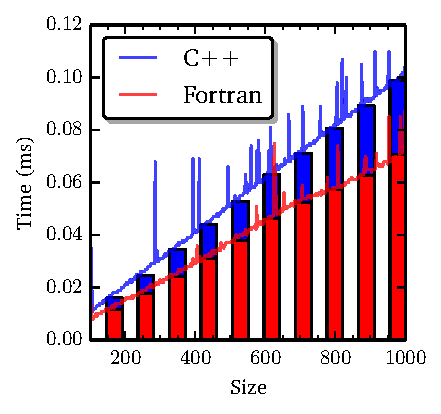
\includegraphics[width=\textwidth]{figs/backmatter/wignerTimes.pdf}
  \caption{Time (in ms) to compute sets of a given size of coupling coefficients, specifically the 
	    $3j$-symbol, in this case.}
 \end{subfigure}\hfill
 \begin{subfigure}[b]{0.5\textwidth}
  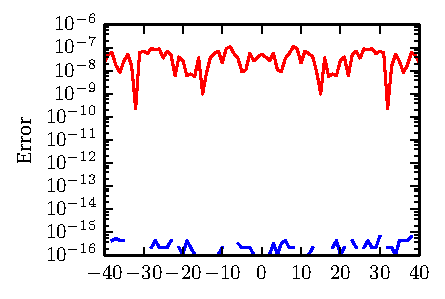
\includegraphics[width=\textwidth]{figs/backmatter/wignerPrecision.pdf}
  \caption{Precision of the Fortran and C++ implementations of the algorithm obtained%
	    by computing the orthogonality relationship \eqref{eq:app.wigner.orthogonality}.}
 \end{subfigure}
 \caption{Performance and precision of our numerical algorithms.}
\end{figure}

\begin{equation}
 \label{eq:app.wigner.orthogonality}
 \sum_{m1,m2} (2l_3+1)\begin{pmatrix} l_1 & l_2 & l_3 \\ m_1 & m_2 & m_3\end{pmatrix}^2=1
\end{equation}


\begin{table}
 \begin{center}
 \newcommand{\A}{$\begin{aligned}A(j_1) &=\left[j_1^2-(j_2-j_3)^2\right]^{1/2}\\&\phantom{=}\times\left[(j_2+j_3+1)^2-j_1^2\right]^{1/2}\\&\phantom{=}\times\left[j_1^2-m_1^2\right]^{1/2}\end{aligned}$}
 \newcommand{\B}{$\begin{aligned}B(j_1) &=-(2j_1+1)\\&\phantom{=}\times\left[j_2(j_2+1)m_1\right.\\&\phantom{=\times}-j_3(j_3+1)m_1\\&\phantom{=\times}\left.-j_1(j_1+1)(m_3-m_2)\right]\end{aligned}$}
 \newcommand{\E}{$\begin{aligned}E(j_1) &=\left\{\left[j_1^2-(j_2-j_3)^2\right]\right.\\&\phantom{=}\times\left[(j_2+j_3+1)^2-j_1^2\right]\\&\phantom{=}\times\left[j_1^2-(j_5-j_6)^2\right]\\&\phantom{=}\times\left.\left[(j_5+j_6+1)^2-j_1^2\right]\right\}^{1/2}\end{aligned}$}
 \newcommand{\F}{$\begin{aligned}F(j_1) &= (2j_1+1)\\&\phantom{=}\times\left\{j_1(j_1+1)\left[--+\right]\right.\\&\phantom{=\times}+j_5(j_5+1)\left[++-\right]\\&\phantom{=\times}+j_6(j_6+1)\left[+-+\right]\\&\phantom{=\times}\left.-2j_1(j_1+1)l_1(l_1+1)\right\}\end{aligned}$}
 \caption{Parameters and coefficients of the three-term recursion relations satisfied
	  by the $3j$- and $6j$-symbols.
	  The expression $[++-]$ represents the coefficient $[j_1(j_1+1)+j_2(j_2+1)-j_3(j_3+1)]$ and similarly for other signs in the bracket.}
 \label{tab:app.wigner.coeffsRecursion}
  \begin{tabular*}{\columnwidth}{m{0.1\textwidth}@{\extracolsep{\fill}}l@{\extracolsep{\fill}}l}
  \hline\hline
  $3j$- or $6j$-symbols	&	 $f(j_1)=\begin{pmatrix} j_1 & j_2 & j_3 \\ m_1 & m_2 & m_3 \end{pmatrix}$ & $h(j_1)=\begin{Bmatrix} j_1 & j_2 & j_3 \\ j_4 & j_5 & j_6 \end{Bmatrix}$\\
  \hline
  $\alpha_\psi$			& $j_1A(j_1+1)$		& $jE(j_1+1)$	\\
  $\beta_\psi$			& $B(j_1)$		& $F(j)$	\\
  $\gamma_\psi$			& $(j_1+1)A(j_1)$	& $(j_1+1)E(j)$	\\
				&			&		\\
  \multirow{4}{*}{Functions}	& \A			& \E		\\
  				&			&		\\
				& \B			& \F		\\
				&			&		\\
 \multirow{2}{*}{Endpoints}	& $j_{1\text{min}}=\text{max}(|j_2-j_3|,|m_1|)$ & $j_{1\text{min}}=\text{max}(|j_2-j_3|,|j_5-j_6|)$	\\
				& $j_{1\text{max}}=j_2+j_3$ 			& $j_{1\text{max}}=\text{min}(j_2+j_3,j_5+j_6)$		\\
				&			&		\\
 Normalization			& $\sum_{j_1}(2j_1+1)f(j_1)^2=1$		& $(2j_4+1)\sum_{j_1}(2j_1+1)h(j_1)^2=1$		\\
 				&			&		\\
 Sign				& $\text{sgn}[f(j_{1\text{max}})]=(-1)^{j_2-j_3-m_1}$ & $\text{sgn}[h(j_{1\text{max}})]=(-1)^{j_2+j_3+j_5+j_6}$\\
  \hline\hline
 \end{tabular*}
 \end{center}
\end{table}


% -- We draw a flowchart of the algorithm. 
% Block styles
\tikzstyle{decision} = [diamond, draw, fill=blue!20,text width=4.5em, text badly centered, node distance=3cm, inner sep=0pt]
\tikzstyle{block} = [rectangle, draw, fill=blue!20, text width=5em, text centered, rounded corners, minimum height=4em]
\tikzstyle{line} = [draw, -latex']
\tikzstyle{cloud} = [draw, ellipse,fill=red!20, node distance=3cm,minimum height=2em]
\tikzstyle{empty} = [fill=white]

% Actual flowchart
\begin{figure}
\begin{center}
\begin{tikzpicture}[scale=0.75,node distance = 2.8cm, auto]
 % -- We place the nodes
 \node [block] (init) {Enforce selection rules};
 \node [decision, below of=init] (sizeSets) {Determine boundaries and size of set};
 \node [block, below of=sizeSets] (size2) {Two-term forward recursion};
 \node [block, left of=size2] (size1) {Use analytical formula};
 \node [block, right of=size2] (otherSize) {Forward recursion};
 \node [decision,below of=otherSize] (overflow){$|\psi(j_1)|>$\\SRHUGE?};
 \node [block, left of=overflow](rescale) {Rescale forward recursion};
 \node [decision,below of=overflow] (monitor) {$|X(j_1)|$ increasing?};
 \node [decision,below of=monitor] (loopDone) {Loop done?};
 \node [block,left of=loopDone] (backward) {Backward recursion until midpoint};
 \node [block,below of=backward] (lambda) {Compute $\lambda$; rescale forward recursion};
 \node [block,right of=lambda] (normalization) {Normalize set of coefficients};
 \node [block, below of=normalization] (return){Return};
 
 % -- We place the edges
 \path [line] (init) -- (sizeSets);
 \path [line] (sizeSets) -| node [near end] {size$=1$} (size1);
 \path [line] (sizeSets) -- node [near start] {size$=2$} (size2);
 \path [line] (sizeSets) -| node [near end] {other sizes} (otherSize);
 \path [line] (otherSize) -- (overflow);
 \path [line] (overflow) -- node[near start]{yes} (rescale);
 \path [line] (overflow) -- node[near start]{no}  (monitor);
 \path [line] (rescale) |- (monitor);
 \path [line] (monitor.south west) -- node[near start]{yes} (backward.north east);
 \path [line] (monitor) -- node[near start]{no} (loopDone);
 \path [line] (loopDone.east) -- node[near start]{no} ($(loopDone.east)+(2,0)$) |- (otherSize.east);
 \path [line] (loopDone) -- node[near start]{yes} (normalization);
 \path [line] (normalization) -- (return);
 \path [line] (backward) -- (lambda);
 \path [line] (lambda) -- (normalization);
 \path [line] (size1) |- (return);
 \path [line] (size2.south) -- ($(size2.south)-(0,1)$) -- ++(-2,0) -- ($(lambda.south)-(2,1)$) -- ++(3,0) -- (normalization.south west);
\end{tikzpicture}
\end{center}
\caption{Flowchart of the algorithm used to compute the coupling coefficients. SRHUGE is the 
	  square root of the biggest representable number in our floating point representation.}
\label{fig:app.wigner.flowchart}
\end{figure}

\section{Spherical Harmonics Transform}
In the variable phase method, we must find the spherical 
harmonics transform, i.e. the spherical moments, of the 
potential. To find these moments, we will have to become
intimate with the spherical harmonics. 

\subsection{Definition of the scalar and vector spherical harmonics}
While there is a number of ways to introduce the spherical harmonics, 
we will take the top to bottom approach: from the general to the specific. 
In all generality, spherical harmonics are solutions of the equation
  \begin{equation}
    \left[\nabla^2_\Omega+\ell(\ell+1)\right]Y^{\ell S}_{jm}(\theta,\varphi)=0
  \end{equation}
where $Y_{jm}^{\ell S}$ is actually a \textit{tensor} spherical harmonic. 
It describes the angular distribution and polarization of spin-$S$ particles 
with angular momentum $j$, projection $m$ and orbital angular momentum $\ell$ \cite{VAR1988}.
While the study of particles with arbitrary spin $S$ is interesting in its own right,
we will concentrate on the case of particles of spin-$1$ and their scalar approximation
(spin-$0$). Since the values of $\ell$ range from $|J-S|$ to $J+S$, the 
spin-$0$ case reduces to the usual scalar spherical harmonics while the spin-$1$
case are the \textit{vector} spherical harmonics. As said in the main text, they 
can be formed by a superposition of scalar spherical harmonics of the form
  \begin{equation}
    \bo{Y}_{jm}^\ell(\theta,\varphi)=\sum_{m',\sigma}C_{lm',1\sigma}^{jm}Y_\ell^{m'}(\theta,\varphi)\hat{\bo{e}}_\sigma
  \end{equation}
The numerical evaluation of these functions are then contingent on the evaluation of the
scalar spherical harmonics and the Clebsch-Gordan coefficients. The first was covered in the 
previous appendix and we will soon tend to the second. 

The scalar spherical harmonics can simply be written as
  \begin{equation}
   Y_{\ell}^m(\theta,\varphi) = P_\ell^m(\cos\theta)e^{im\varphi}
  \end{equation}
where $P_\ell^m$ is the normalized version of the associated 
Legendre polynomials \cite{PRE2007}. They are related to
the usual Legendre polynomials $\widetilde{P}_\ell^m$ through
  \begin{equation}
    P_\ell^m(x) = \sqrt{\frac{2\ell+1}{4\pi}\frac{(\ell-m)!}{(\ell+m)!}}\widetilde{P}_\ell^m(x)
  \end{equation}
To numerically evaluate the spherical harmonics, then, we must safely 
evaluate the associated Legendre polynomials. One of the only 
stable recurrence relation is \cite{PRE2007}
  
  \begin{equation}
   P_\ell^m(x)=\sqrt{\frac{4l^2-1}{l^2-m^2}}\left[xP_{\ell-1}^m(x)-\sqrt{\frac{(l-1)^2-m^2)}{4(l-1)^2-1}}P_{\ell-2}^m(x)\right]
  \end{equation}
The initial conditions are provided by 
  \begin{align}
   P_m^m(x)	&=(-1)^m\sqrt{\frac{2m+1}{4\pi(2m)!}}(2m-1)!!(1-x^2)^{m/2}	\\
   P_{m+1}^m(x)	&=x\sqrt{2m+3}P_m^m(x)
  \end{align}
At first sight, it might seem dangerous to evaluate 
$P_m^m(x)$ because of the division of two factorial functions. 
However, by taking the square of the expression and looking
at the factorial functions, we have
  \begin{equation}
   a_m = \frac{[(2m-1)!!]^2}{(2m)!}.
  \end{equation}
This can evaluated rather simply by noting that $(2m-1)!!=\nicefrac{(2m)!}{2^mm!}$.
Rearranging, we get
  \begin{equation*}
   a_m = \frac{(2m)!}{2^{2m}(m!)^2} = \frac{1}{2^{2m}}\binom{2m}{m}.
  \end{equation*}
We further notice that
  \begin{equation}
   \frac{a_{m+1}}{a_m} = \frac{2^{2m}}{2^{2(m+1)}}\frac{\binom{2(m+1)}{m+1}}{\binom{2m}{m}}=\frac{2m+1}{2m+2}.
  \end{equation}
We can then safely evaluate $P_m^m(x)$ using the formula
  \begin{equation}
   P_m^m(x) = \sqrt{\frac{2m+1}{4\pi}\prod_{i=0}^{m-1}\frac{2i+1}{2i+2}(1-x^2)}.
  \end{equation}

Our numerical implementation shows machine precision for all spherical
harmonics up to $\ell=3$ (we compared the results of our algorithm 
with the analytical forms of the spherical harmonics).  Moreover, we 
tested our algorithm against the following sums \cite[\S 5.10]{VAR1988}
  \begin{align}
   \sum_{m} \left|Y_\ell^m(\theta,\varphi)\right|^2	&= \frac{2\ell+1}{4\pi}	\label{eq:app.sph.sum1}\\
   \sum_m m\left|Y_\ell^m(\theta,\varphi)\right|^2 	&= 0			\label{eq:app.sph.sum2}\\
   \sum_m m^2\left|Y_\ell^m(\theta,\varphi)\right|^2	&= \frac{\ell(\ell+1)(2\ell+1)}{8\pi}\sin^2\theta.\label{eq:app.sph.sum3}
  \end{align}
They are verified to a precision of $10^{-7}$ up to $\ell=500$. The uncertainty
on the sums grows with $\ell$. Figure \ref{fig:app.sph.precision} tells us 
that the spherical harmonics are computed near to or at machine precision
(in \texttt{double}). The increasing error is due to error accumulation. 
At large $\ell$, there are a lot of terms to sum, thus increasing
the absolute error made in the computation. 

\subsection{Spherical Harmonics Transform}
While the Fast Fourier Transform has had hundreds
of experts working on it, this is not true of the 
Fast Spherical Harmonics Transform. The program libraries
are scarce and, for the most part, still in their infancy. 
This is in sharp contrast with the FFT case, where numerous 
libraries provide algorithms that performs FFTs at a cost 
of $\mathcal{O}(n\log n)$. \texttt{FFTW} is an example of such a mature, 
robust program library.

Any smooth function can be expanded in a spherical harmonics
series (they form a complete basis on the 2-sphere) with \cite[\S 6.7.1]{PRE2007}
  \begin{equation}
    f(\theta,\varphi) = \sum_{\ell=0}^{\ell_\text{max}}\sum_{m=-\ell}^\ell a_{\ell m}P_\ell^m(\cos\theta)e^{im\varphi}
  \end{equation}
Using the orthonormality conditions, we can find an expression for the expansion coefficients
  \begin{equation}
   a_{\ell m} = \mathop{\iint}_\Omega f(\theta,\varphi)e^{-im\varphi}P_\ell^m(\cos\theta)\sin\theta d\theta d\varphi
  \end{equation}
In the discrete case, then, the integral becomes a quadrature
  \begin{equation}
   a_{\ell m} = \sum_{i,j}w(\theta_i)f(\theta_i,\varphi_j)e^{-im\varphi_j}P_\ell^m(\cos\theta_i).
  \end{equation}
The fastest way to perform the quadrature over $\varphi_j$ is, of course, to use
the FFT. We will perform the quadrature over $\theta_i$ by using a Gauss-Legendre
quadrature. While the cost of such an algorithm is the worst we could get ($\mathcal{O}(\ell^3)$), 
it is also the easiest to implement. Faster transforms are available in the literature \cite{TYG2006,TYG2008,TYG2010}.

To find the abscissas of the Gauss-Legendre quadrature (the roots
of $P_\ell^0(\cos\theta)$), we perform a few rounds of Newton-Raphson 
using the following initial guess on the positions of the zeros \cite{ABR1965}
  \begin{equation}
   \xi_{\ell,k} = \left(1-\frac{1}{8\ell^2}+\frac{1}{8\ell^3}\right)\cos\left(\frac{4k-1}{4\ell+2}\pi\right)+\mathcal{O}\left(\ell^{-4}\right)
  \end{equation}
where $\xi_{\ell,k}$ is the $k$th root (ordered in $[-1,1]$) of $P_\ell^0(\cos\theta)$.

\begin{figure}
 \centering
 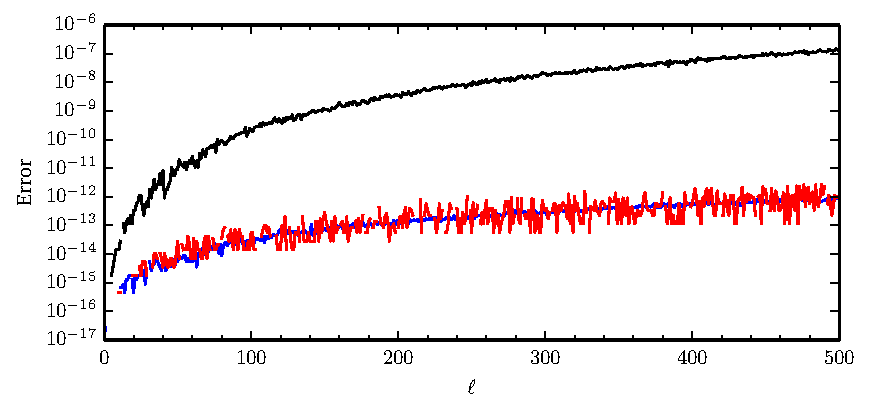
\includegraphics[width=0.9\textwidth]{figs/backmatter/SphPrecision.pdf}
 \caption[Precision of our implementation of the algorithm that evaluates the spherical harmonics]
	  {Precision of our implementation of the algorithm that evaluates the spherical harmonics. 
	  The {\color{blue} blue} curve corresponds to \eqref{eq:app.sph.sum1}, the 
	  {\color{red} red} curve to \eqref{eq:app.sph.sum2} and the black curve to 
	  \eqref{eq:app.sph.sum3}.}
 \label{fig:app.sph.precision}
\end{figure}

 \nocite{*}